%&latex
% Copyright 2011 Ruslan Kiyanchuk (c) <ruslan.kiyanchuk@gmail.com>
% 
% 
%/

\chapter{PERSPECTIVE LIGHTWEIGHT CIPHER PROPERTIES ANALYSIS AND REQUIREMENTS}
\label{sec:lightweight}

\section{PRESENT cipher description}

Confidentiality of data transfer in modern information and telecommunication
systems is usually provided by application of symmetric block ciphers.  At the
same time widely used block ciphers are generally designed for software
implementation (AES) or special-purpose hardware modules (DES, TripleDES).
Their system-on-a-chip implementations with strict constraints to the number of
logic gates and energy consumption are quite ineffective.  Financial
applications, wireless sensor networks, RFID tags, electronic toll collection
systems, all require secure data processing, ensuring its integrity and
confidentiality~\cite{lwc:poschmann:2007}.  Consequently, such systems require a
new generation cryptographic algorithms.

This chapter examines requirements for block ciphers designed for lightweight
hardware implementations, describes the perspective cipher specifications,
its properties and comparison with already existing ciphers.

Vast majority of modern symmetric block ciphers are designed for software
implementation while the hardware implementations require intense computing
resources (gates, area on a chip, frequency and energy consumption) for
attaining acceptable efficiency. Harshly constrained pervasive devices
capabilities do not allow the effective usage of existing reliable
ciphers~\cite{lwc:wireless:seys}.

Thereby, the need for developing perspective symmetric block ciphers designed
for effective hardware implementation and assuring moderate security level
emerged.  One of the latest findings in this area is PRESENT cipher
designed for hardware implementation on constrained devices.


The main goal when designing PRESENT was moderate security level,
implementation efficiency and simplicity. It may be used on ultra constrained
hardware when utilization of existing ciphers such as AES is impossible.
The hardware PRESENT implementation requires only $ 1000 $ gate
equivalents (GE)~\cite{secsi:2007}.

Cipher developments with the same targets in mind had already taken place
earlier. HIGHT was published in
2006~\cite{DBLP:conf:ches:HongSHLLKLCLJKKC06}. It consists of a Feistel network
and only 8-bit operations, has 64 bit input block size, 128 bit key length and
32 rounds. Its authors claim the hardware implementation to fit on $ 3048 $ gate
equivalents.

The mCrypton cipher was published in 2006 and intended for both software
and hardware implementations. It has 64-bit input block and consists of 13 rounds.
The possible key length is 64, 96 or 128 bits. The hardware implementation of
enciphering function requires at least $ 2420 $ gate equivalents.

Scalable Encryption Algorithm (SEA) was proposed in 2006 and targeted for
constrained (software) devices with special emphasis on scalability~\cite{sea}.
Therefore SEA has a wide range of deployment. The input block size $ n $,
key length $ k $, machine word $ b $ and number of rounds $ nr $ are variable
cipher parameters. The price for such scalability is implementation complexity
that requires $ 3758 $ GE with $ n = 96 $ bit, $ b = 8 $ bit, $ nr = 93 $.

\subsection{Perspective block cipher requirements for hardware \mbox{implementation}}

PRESENT designers set the following requirements for the cipher \cite{ches:present:2007}:
\begin{itemize}
    \setlength{\itemsep}{0pt}%
        \setlength{\parskip}{0pt}%
    \item the cipher is to be implemented in hardware;
    \item applications will only require moderate security levels;
    \item applications are unlikely to require the encryption of large amounts
        of data; implementations might therefore be optimised for performance or
        for space without too much practical impact;
    \item in some applications it is possible that the key will be fixed at the
        time of device manufacture; in such cases there would be no need to
        re-key a device (which would incidentally rule out a range of key
        manipulation attacks);
    \item after security, the physical space required for an implementation will
        be the primary consideration; this is closely followed by peak and
        average power consumption, with the timing requirements being a third
        important metric;
    \item in applications that demand the most efficient use of space, the block
        cipher will often only be implemented as encryption-only; in this way it
        can be used within challenge-response authentication protocols and,
        with some careful state management, it could be used for both encryption
        and decryption of communications to and from the device by using the
        counter mode.
\end{itemize}

PRESENT is a symmetric block cipher with 64 bit input block size and 80 bit
key length needed for assuring moderate security level. This is also the
position taken for hardware profile stream ciphers submitted to eSTREAM
project~\cite{estream}. Specification also defines a 128 bit key. The
PRESENT encipher and decipher hardware implementation still requires less
space than AES encipher-only implementation~\cite{lwc:lounge}. The round
keys can be computed on the fly during enciphering (each subkey per round, since
round key computation consists in updating the key register).

PRESENT is a substitution-permutaion network (SPN) and contains 31 rounds
(fig.~\ref{fig:present-cipher}).
The last 32-nd subkey is used for whitening after main loop. The loop consists
of linear bit permutation layer and nonlinear substitution layer. The nonlinear
layer uses 4-bit S-box which is applied 16 times to the whole input block each
round. Key is injected into data via modulo 2 addition.

\begin{figure}[htbp]
    \centering
    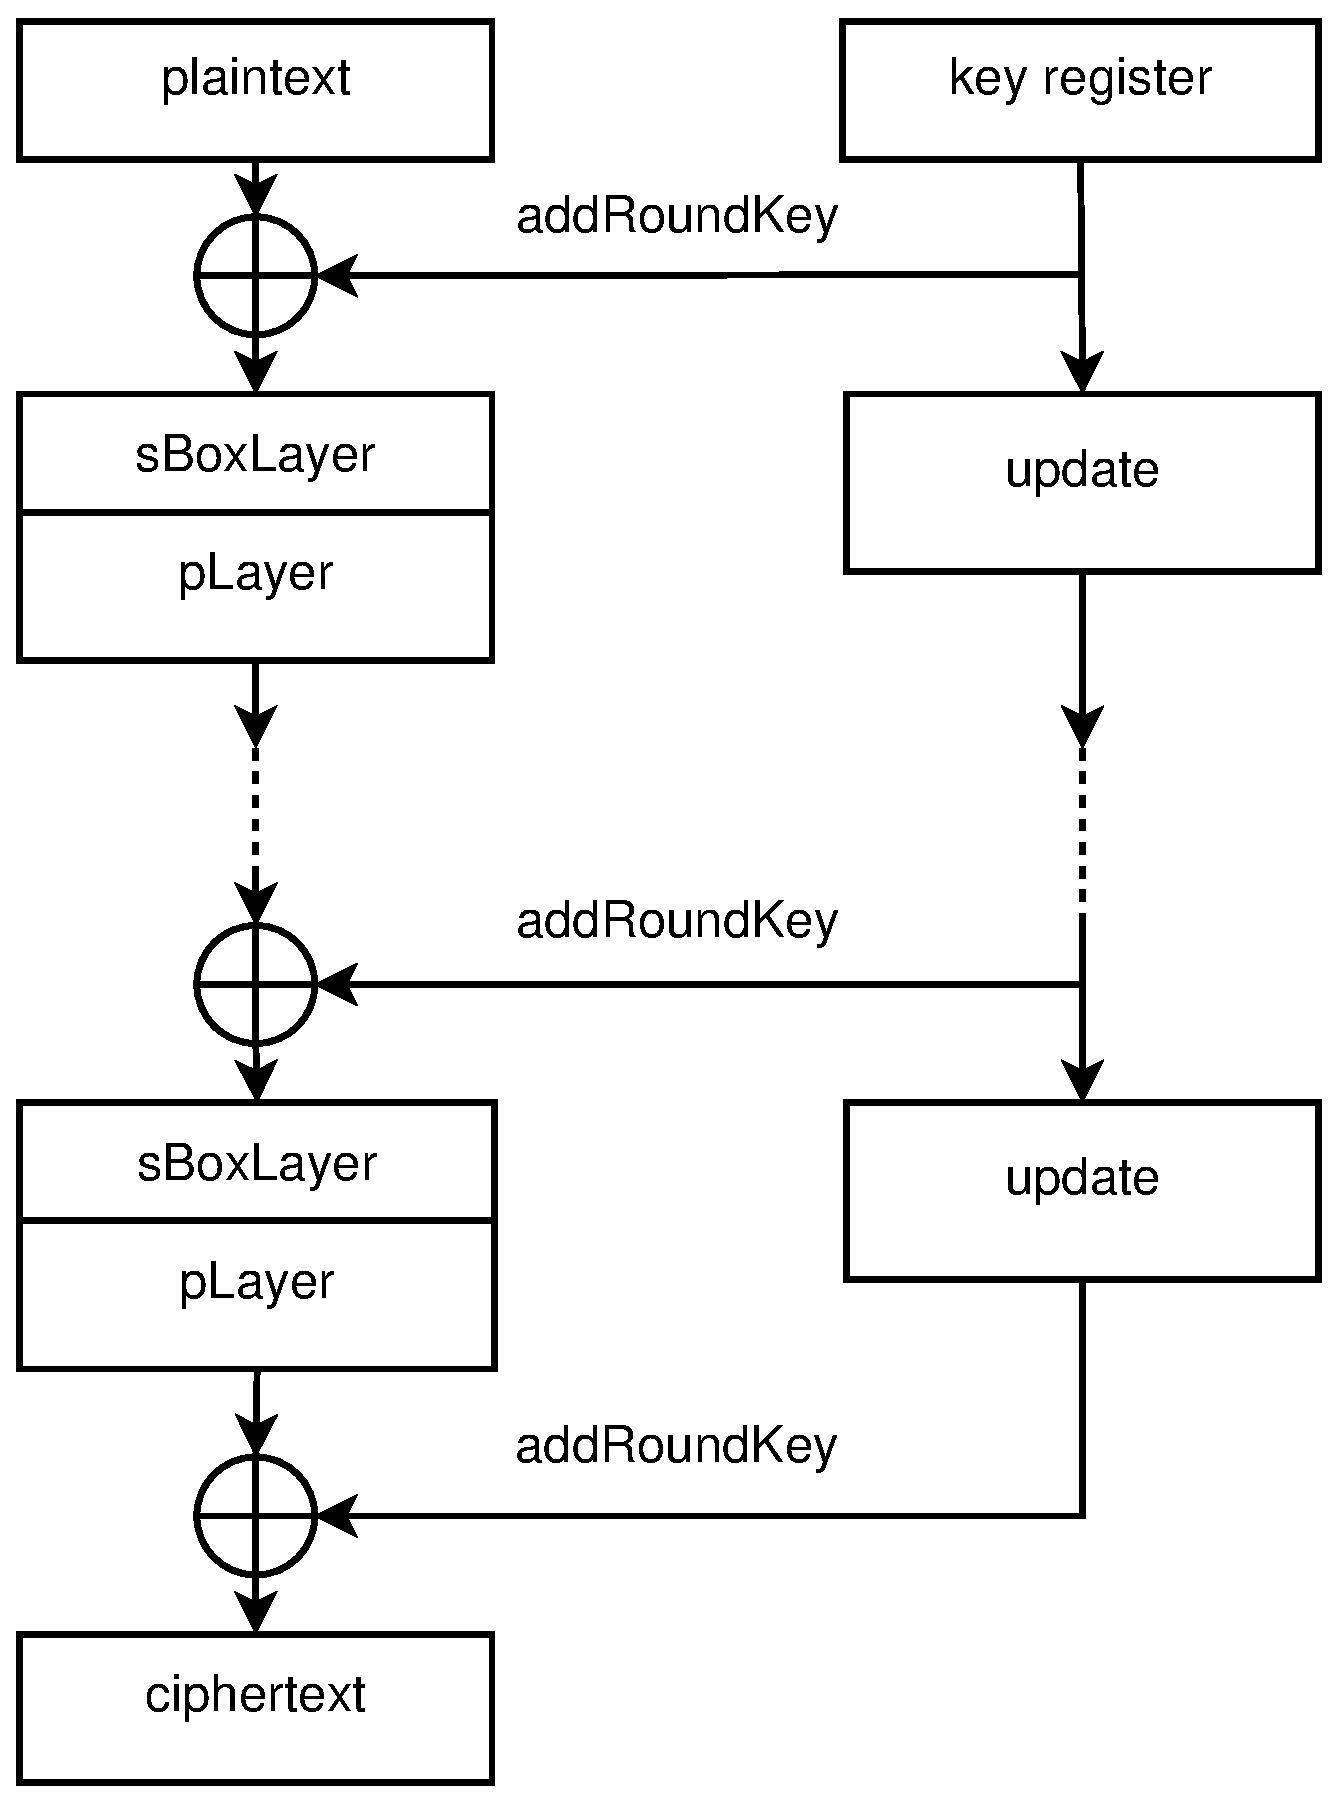
\includegraphics[scale=0.4]{cipher}
    \caption{PRESENT enciphering}
    \label{fig:present-cipher}
\end{figure}

\subsection{Substitution layer}

The nonlinear layer is represented by a single 4-bit substitution 
$ F_2^4 \rightarrow F_2^4 $. It is a direct outcome of strict constrains on
efficiency and implementation area. Some additional restrictions are applied on
S-box for reaching an avalanche effect. Let us denote the Fourier coefficient of
$ S $ by
\begin{equation}
    S_b^W(a) = \sum\limits_{x \in F_2^4} (-1)^{(b,  S(x)) + (a,  x)}.
\end{equation}

Than the PRESENT S-box (table~\ref{tbl:sbox}) meets the following
conditions:
\begin{enumerate}
    \setlength{\itemsep}{0pt}%
        \setlength{\parskip}{0pt}%
    \item for any fixed non-zero input difference  
        $ \Delta_I \in F_2^4 $ and any fixed non-zero output difference 
        $ \Delta_O \in F_2^4 $ it is required that
        \begin{equation}
            \# \left\{ x \in F_2^4 \, | \, S(x) + S(x + \Delta_I) = \Delta_O \right\}
            \leq 4;
        \end{equation}
    \item for any fixed non-zero input difference
        $ \Delta_I \in F_2^4 $ and any fixed output difference
        $ \Delta_O \in F_2^4 $ such that
        $ wt(\Delta_I) = wt(\Delta_O) = 1 $ the following is true
        \begin{equation}
            \# \left\{ x \in F_2^4 \, | \, S(x) + S(x + \Delta_I) = \Delta_O\ \right\} = 0;
        \end{equation}
    \item for all non-zero $ a \in F_2^4 $ and all non-zero $ b \in F_2^4 $
        it holds that $ \left| S_b^W (a) \right| \leq 8 $;
    \item for all $ a \in F_2^4 $ and all non-zero $ b \in F_2^4 $ such that
        $ wt(a) = wt(b) = 1 $ it holds that $ \left| S_b^W (a) \right| \leq 4 $.
\end{enumerate}
\begin{table}[p]
    \caption{PRESENT S-box}
    \label{tbl:sbox}
    \small
    \centering
    \begin{tabular}{|c||c|c|c|c|c|c|c|c|}
        \hline
        $ x $ & 0 & 1 & 2 & 3 & 4 & 5 & 6 & 7 \\ \hline
        $S[x]$& C & 5 & 6 & B & 9 & 0 & A & D \\ \hline
        $x$ & 8 & 9 & A & B & C & D & E & F \\ \hline
        $S[x] $ & 3 & E & F & 8 & 4 & 7 & 1 & 2 \\ \hline
    \end{tabular}
\end{table}
From entire set of S-boxes satisfying the specified conditions the one was chosen
with the most efficient hardware implementation (that is less logic gates
required for boolean representation). The boolean function of each S-box bit
after minimization is showed below: 

\noindent
$ S_0(x) = x_3 \cdot x_2 \cdot \overline{x_1} \cdot x_0 +
\overline{x_3} \cdot x_2 \cdot \overline{x_1} \cdot \overline{x_0} + 
\overline{x_3} \cdot \overline{x_2} \cdot \overline{x_1} \cdot x_0 +
x_3 \cdot x_1 \cdot \overline{x_0} + 
\overline{x_3} \cdot x_2 \cdot x_1 \cdot x_0 + 
\overline{x_3} \cdot \overline{x_2} \cdot x_1 \cdot x_0 +
x_3 \cdot \overline{x_2} \cdot \overline{x_0} $; 

\noindent
$ S_1(x) = \overline{x_3} \cdot x_2 \cdot x_1 \cdot \overline{x_0} + x_3 \cdot  
x_2 \cdot x_0 + \overline{x_2} \cdot {x_1} \cdot \overline{x_0} + x_3 \cdot 
\overline{x_2} \cdot \overline{x_1} \cdot x_0 + \overline{x_3} \cdot 
\overline{x_2} \cdot x_1 \cdot x_0 + x_3 \cdot \overline{x_2} \cdot
\overline{x_0} $;

\noindent
$ S_2(x) = \overline{x_3} \cdot \overline{x_2} \cdot \overline{x_1} \cdot
\overline{x_0} + \overline{x_3} \cdot \overline{x_2} \cdot \overline{x_1} \cdot 
x_0 + x_3 \cdot x_2 \cdot \overline{x_1} + \overline{x_3} \cdot x_2 \cdot x_1
\cdot x_0 + \overline{x_2} \cdot x_1 \cdot \overline{x_0} + x_3 \cdot
\overline{x_2} \cdot \overline{x_1} \cdot x_0 $;

\noindent
$ S_3(x) = \overline{x_3} \cdot x_2 \cdot x_1 \cdot \overline{x_0} +
\overline{x_3} \cdot \overline{x_2} \cdot \overline{x_1} \cdot \overline{x_0} +
\overline{x_3} \cdot x_2 \cdot \overline{x_1} \cdot \overline{x_0} + x_3 \cdot
\overline{x_2} \cdot x_1 + \overline{x_3} \cdot x_2 \cdot x_1 \cdot x_0 + x_3
\cdot \overline{x_2} \cdot \overline{x_1} \cdot x_0 + \overline{x_3} \cdot
\overline{x_2} \cdot x_1 \cdot x_0 $;

\noindent where $ \overline{x_i} $ denotes the inversion of $ x_i $ bit, 
$ \cdot $ denotes logical \verb+AND+, $ + $ denotes logical \verb+OR+.

\subsection{Permutation layer}

The main problem considered during the permutation layer
(table~\ref{tbl:player}) development was the number of required logic gates for
implementation. Functional representation of permutation is showed in formula
(\ref{eqn:player}).
\begin{equation}
    \label{eqn:player}
    P(i) = \left\{
    \begin{array}{ll}
        i \cdot 16 \mod 63, & i \in {0, \hdots, 62} \\
        63,  & i = 63.
    \end{array} \right.
\end{equation}

\begin{table}[p]
    \centering
    \caption{PRESENT permutation layer}
    \small
    \label{tbl:player}
    \begin{tabular}{|c||c|c|c|c|c|c|c|c|}
        \hline
        $ i $  & 0  & 1  & 2  & 3  & 4 & 5  & 6  & 7  \\[-0.8ex]
        $P(i)$ & 0  & 16 & 32 & 48 & 1 & 17 & 33 & 49 \\
        \hline
        $ i $  & 8 & 9  & 10 & 11 & 12 & 13 & 14 & 15 \\[-0.8ex] 
        $P(i)$ & 2 & 18 & 34 & 50 & 3  & 19 & 35 & 51 \\ 
        \hline

        $ i $  & 16 & 17 & 18 & 19 & 20 & 21 & 22 & 23 \\[-0.8ex]
        $P(i)$ & 4  & 20 & 36 & 52 & 5  & 21 & 37 & 53 \\
        \hline
        $ i $  & 24 & 25 & 26 & 27 & 28 & 29 & 30 & 31 \\[-0.8ex]
        $P(i)$ & 6  & 22 & 38 & 54 & 7  & 23 & 39 & 55 \\ 
        \hline

        $ i $  & 32 & 33 & 34 & 35 & 36 & 37 & 38 & 39 \\[-0.8ex] 
        $P(i)$ & 8  & 24 & 40 & 56 & 9  & 25 & 41 & 57 \\
        \hline
        $ i $  &  40 & 41 & 42 & 43 & 44 & 45 & 46 & 47 \\ [-0.8ex] 
        $P(i)$ &  10 & 26 & 42 & 58 & 11 & 27 & 43 & 59 \\ 
        \hline
        $ i $  & 48 & 49 & 50 & 51 & 52 & 53 & 54 & 55 \\[-0.8ex] 
        $P(i)$ & 12 & 28 & 44 & 60 & 13 & 29 & 45 & 61 \\
        \hline
        $ i $  & 56 & 57 & 58 & 59 & 60 & 61 & 62 & 63 \\ [-0.8ex] 
        $P(i)$ & 14 & 30 & 46 & 62 & 15 & 31 & 47 & 63 \\     
        \hline
    \end{tabular}
\end{table}

\subsection{The key schedule}

User key is stored in register $ K $ and is represented with a bit sequence
$ k_{79} k_{78} \hdots k_0 $. Each round the subkey consists of 64 most
significant (left) key register bits. After extracting another subkey the key
register state is updated as follows:
\begin{enumerate}
    \setlength{\itemsep}{1pt}
        \setlength{\parskip}{0pt}
        \setlength{\parsep}{0pt}
    \item $ [k_{79} k_{78} \hdots k_1 k_0] = [k_{18} k_{17} \hdots k_{20} k_{19}] $;
    \item $ [K_{79} k_{78} k_{77} k_{76}] = S[k_{79} k_{78} k_{77} k_{76}] $;
    \item $ [k_{19} k_{18} k_{17} k_{16} k_{15}] = [k_{19} k_{18} k_{17} k_{16}
        k_{15} \oplus \text{round\_counter}] $.
\end{enumerate}

\subsection{Deciphering}

Deciphering uses analogous inverse permutations. Subkeys are supplied in the
same order as during enciphering. The reverse S-box is showed in
table~\ref{tbl:invsbox}.
\begin{table}[hbp]
    \caption{Inverse S-box of PRESENT}
    \label{tbl:invsbox}
    \small
    \centering
    \begin{tabular}{|c||c|c|c|c|c|c|c|c|}
        \hline
        $ x $ & 0 & 1 & 2 & 3 & 4 & 5 & 6 & 7 \\
        \hline
        $S[x]$& 5 & E & F & 8 & C & 1 & 2 & D \\
        \hline
        $x$ & 8 & 9 & A & B & C & D & E & F \\
        \hline
        $S[x]$ & B & 4 & 6 & 3 & 0 & 7 & 9 & A \\ 
        \hline
    \end{tabular}
\end{table}
Inverse permutation layer is showed in table~\ref{tbl:invplayer}.
\begin{table}[p]
    \centering
    \caption{PRESENT inverse permutation layer}
    \label{tbl:invplayer}
    \small
    \begin{tabular}{|c||c|c|c|c|c|c|c|c|}
        \hline
        $ i $  & 0 & 1 & 2 & 3  & 4  & 5  & 6  & 7  \\[-0.8ex]
        $P(i)$ & 0 & 4 & 8 & 12 & 16 & 20 & 24 & 28 \\
        \hline
        $ i $  & 8  & 9  & 10 & 11 & 12 & 13 & 14 & 15 \\[-0.8ex]  
        $P(i)$ & 32 & 36 & 40 & 44 & 48 & 52 & 56 & 60 \\        
        \hline
        $ i $  & 16 & 17 & 18 & 19 & 20 & 21 & 22 & 23 \\[-0.8ex]
        $P(i)$ & 1  & 5  & 9  & 13 & 17 & 21 & 25 & 29 \\
        \hline
        $ i $  & 24 & 25 & 26 & 27 & 28 & 29 & 30 & 31 \\[-0.8ex] 
        $P(i)$ & 33 & 37 & 41 & 45 & 49 & 53 & 57 & 61 \\       
        \hline
        $ i $  & 32 & 33 & 34 & 35 & 36 & 37 & 38 & 39 \\[-0.8ex]
        $P(i)$ & 2  & 6  & 10 & 14 & 18 & 22 & 26 & 30 \\
        \hline
        $ i $  & 40 & 41 & 42 & 43 & 44 & 45 & 46 & 47 \\[-0.8ex] 
        $P(i)$ & 34 & 38 & 42 & 46 & 50 & 54 & 58 & 62 \\       
        \hline
        $ i $  & 48 & 49 & 50 & 51 & 52 & 53 & 54 & 55 \\[-0.8ex]
        $P(i)$ & 3  & 7  & 11 & 15 & 19 & 23 & 27 & 31 \\
        \hline
        $ i $  & 56 & 57 & 58 & 59 & 60 & 61 & 62 & 63 \\[-0.8ex] 
        $P(i)$ & 35 & 39 & 43 & 47 & 51 & 55 & 59 & 63 \\               
        \hline
    \end{tabular}
\end{table}

\section{PRESENT hardware implementation properties}

Cipher authors considered a wide variety of different target platforms ranging
from highly-optimized ASICs, over more flexible but still efficient low-cost
FPGAs to hardware-software co-design approaches and flexible software
implementations for 4-, 8-, 16- and 32-bit processors.

We will investigate the ASIC implementation as it is the most efficient one.

\subsection{Performance evaluation}

To assess the efficiency of implementation the developers used the following
metrics presented in table~\ref{tbl:lwc-dev-metrics}.

\begin{table}[htbp]
\centering
\caption{Development metrics for lightweight cipher}
\label{tbl:lwc-dev-metrics}
\begin{tabular}{|c|p{0.8\textwidth}|} \hline
    Area &
    Area requirements are usually measured in $ \mu m^2 $ , but this
    value depends on the fabrication technology and the standard cell
    library. In order to compare the area requirements independently it is
    common to state the area as gate equivalents [GE]. One GE is equivalent
    to the area which is required by the two-input NAND gate with the
    lowest driving strength of the appropriate technology. The area in GE is
    derived by dividing the area in $ \mu m^2 $ by the area of a two-input NAND
    gate.  \\ \hline
    Cycles & 
    Number of clock cycles to compute and read out the result. \\ \hline
    Time &
    The required amount of time for a certain operation can be
    calculated by dividing the amount of cycles by the operating 
    $ t = \frac{cycles}{freq} $. \\ \hline
    Throughput &
    The rate at which new output is produced with respect to
    time. The number of output bits is divided by the time, i.e. by the
    needed cycles and multiplied by the operating frequency. It is expressed
    in bits per second [bps]. \\ \hline
    Power &
    The power consumption is estimated on the gate level by
    Synopsys \verb+PowerCompiler+. It is provided in micro Watt $ [\mu W] $. \\ \hline
    Energy &
    The energy consumption denotes the power consumption over a
    certain time period.  It can be calculated by multiplying the power
    consumption with the required time of the operation. The energy
    consumption is provided in micro Joule $ [\mu J] $. \\ \hline
    Current &
    The power consumption divided by the typical core voltage. \\ \hline
    Efficiency &
    The area to throughput ratio is used as a measure of
    hardware efficiency. The hardware efficiency is calculated by dividing
    the area requirements by the throughput and is expressed in gate
    equivalents per bits per second $ \left[ \frac{GE}{bps} \right]$. \\ \hline
\end{tabular}
\end{table}

\subsection{Measurements}

Measurements of ASIC round-based PRESENT implementation on 180 nm manufacturing
technology with 4-bit datapath are done at 100 kHz frequency and presented below:

\begin{description}
    \setlength{\itemsep}{1pt}
        \setlength{\parskip}{0pt}
        \setlength{\parsep}{0pt}
    \item[throughput:] 11.7 Kbps;
    \item[area:] $ 1075 $ GE;
    \item[efficiency:] $ 10.89 $ $ \frac{bps}{GE} $;
    \item[current:] $ 2.78 $ $ \mu A $.
\end{description}

Serialized and parallelized architectures implementation is also possible and
described by authors in detail~\cite{secsi:2007}.

\subsection{Cryptographic security}

The substitution layer has been developed with the resistance to differential
and linear cryptanalysis in mind.
The maximum differential probability of a PRESENT S-box is $ 2^{-2} $ and so the
probability of a single 25-round differential characteristic is bounded by $
2^{-100} $.

Differential properties of the S-box are shown in
table~\ref{tbl:present-sbox-diff}.
\begin{table}[htbp]
    \centering
    \caption{PRESENT S-box differential properties}
    \label{tbl:present-sbox-diff}
    \begin{tabular}{|c|c|} \hline
        Differential & Number of occurrences \\ \hline
        0  &  159 \\ \hline
        2  &  72  \\ \hline
        4  &  24  \\ \hline
    \end{tabular}
\end{table}

Linear properties of the S-box are shown in table~\ref{tbl:present-sbox-lin}.
\begin{table}[htbp]
    \centering
    \caption{PRESENT S-box linear properties}
    \label{tbl:present-sbox-lin}
    \begin{tabular}{|c|c|} \hline
        Linear bias & Number of occurrences \\ \hline
        0 & 123 \\ \hline
        2 & 96  \\ \hline 
        4 & 36  \\ \hline 
    \end{tabular}
\end{table}

For approximating 28 cipher rounds with linear cryptanalysis one needs to obtain
$ 2^{84} $ \mbox{plaintext/ciphertext} pairs, which exceeds the set of all
possible plaintexts for PRESENT.

Integral attack on 7-round PRESENT requires $ 2^{43.3} $ chosen
plaintexts, has time complexity $ 2^{100.1} $ and requires $ 2^{77} $ bytes of
memory.

For applying an algebraic attack $ 11067 $ quadratic equations with $ 4216 $
variables have to be solved. Solving such equations is an NP-hard task.
Despite the successful attacks on small-scale versions of block ciphers the
increase of input block size results in enormous time and memory complexity.

The cipher security depends on key scheduling scheme. PRESENT uses round
counter XORing with key register to decrease the correlation between subkeys.
For the sake of nonlinearity while generating key material some bits pass
through S-box when the key register updates (table~\ref{tbl:sbox}). 

All bits in the key register are a nonlinear function of the 80-bit master key
by round 21. Each bit in the key register after round 21 depends on at least
four of the master key bits

By deriving $ K_{32} $, six bits are degree two expressions of the 80 master key
bits, 24 bits are of degree three, while the remaining bits are degree six or
degree nine function of the master key bits.

The statistical saturation attack can break 14 out of 31 rounds of
PRESENT and requires $ 2^{34} $ \mbox{plaintext/ciphertext}
pairs~\cite{collard:present}.

Side channel attacks as well as invasive attacks may be a threat for
PRESENT just like for any other cryptographic primitives.

\section{Comparison of PRESENT, GOST 28147-89 and AES}
\label{sec:lwc-comparison}

Advanced Encryption Standard (AES) is a symmetric block cipher, adopted
as the national encryption standard in USA. This algorithm is widely used in
the world and therefore very well researched.

GOST~28147-89 is a symmetric block cipher recommended for application in
Ukraine, it is also the encryption standard in Russia and other CIS countries,
adopted in 1989.The most efficient known attack breaks the cipher
only $ 2^8 $ times faster than a brute force. In 2010 the
GOST cipher was submitted to ISO to become also an international
standard. For a more detailed description of the cipher refer to
section~\ref{sec:algebraic-gost}.

In consideration of long-term analysis and wide usage of AES and
GOST~28147-89 the comparison of PRESENT with these ciphers is
necessary.

\subsection{Implementation complexity}

The PRESENT structure is incredibly simple. After some precomputations
the algorithm may be replaced with the lookup table and key addition. All cipher
operations can be successfully performed on 4-bit processor and do not require
complex calculations. The most compact implementation requires $ 1000 $ gate
equivalents.

AES has complex structure~\cite{daemen:rijndael}. It uses 8-bit S-box and
its storage requires significantly more memory than 4-bit S-box. For linear bit
diffusion the maximum distance separable (MDS) code based permutation is used.
MDS-permutation uses matrix multiplications in $ GF(2^8) $ and requires
substantial computer resources or additional precomputed lookup tables. Hardware
implementation fits on $ 3100 $ GE on 350 nm manufacturing process.

GOST~28147-89 represents a Feistel network. The cipher uses following
operations: modulo 32 addition, bitwise exclusive \verb+OR+, bitwise shift and a
substitution box. Software implementation for 32-bit processors overtops
PRESENT in throughput. The hardware implementation requires only $ 800 $
gate equivalents~\cite{poschmann:gost}.

\subsection{Cryptographic security}

AES has 128-bit input block size and possible key length of 128, 192 or
256 bits. Number of rounds depends on the key length (10, 12 or 14). Best known
attack on AES-256 has $ 2^{99.5} $ complexity but isn't applicable to
AES-128. Side channel attacks on some implementations might have less
complexity.

GOST~28147-89 has 64-bit input block size and the key length of 256 bits. 
Attack proposed by Nicolas Courtois requires $ 2^{64} $
\mbox{plaintext/ciphertext} pairs and speeds up cryptanalysis only by a factor
of $ 2^8 $ comparable to brute force~\cite{Courtois:cryptoeprint_2011}. It is worth noting,
however, that any cipher can be broken by generating a dictionary of
\mbox{plaintext/ciphertext} values for all possible inputs. Taking into account
the efficiency of PRESENT and its 64-bit input block size it is possible
to compute all \mbox{plaintext/ciphertext} pairs for foreseeable time using
appropriate computing powers.

In distinction from the described ciphers PRESENT has 80 bit key length.
The cipher is inapplicable for enciphering large data requiring high security level, but is
well suited for embedded devices and RFID tags where the moderate security level
for small data sequences is acceptable.

By comparison results GOST~28147-89 is also well suited for such
applications and betters PRESENT on some parameters.

\subsection{Efficiency}

Ciphers efficiency comparison is showed in table~\ref{tbl:comparison}. It is
worth noting that the examined PRESENT implementation described in~\cite{cryptoeprint:2009_516} is designed for
4-bit processor (handles 4 bits per tick) whereas AES and GOST are
unable to function on 4-bit processors. Data for GOST throughput values have
been extrapolated from the author's software implementation benchmarks and
normalized according to the described hardware characteristics
in~\cite{cryptoeprint:2009_516}, so the accuracy has some is not perfect.
\begin{table}[htbp]
    \centering
    \caption{Efficiency comparison of PRESENT, AES and GOST 28147}
    \label{tbl:comparison}
    \begin{tabular}{|l|p{1.5cm}|p{2cm}|p{2.8cm}|p{2.5cm}|p{2cm}|}
        \hline
        Cipher & Key & Block & Throughput, Kb/s & Area, GE & Eff., $\frac{bps}{GE}$ \\
        \hline
        GOST    & 256 & 64  & 14   & 800  & 17.5  \\
        \hline
        AES     & 128 & 128 & 80   & 3100 & 25.81 \\
        \hline
        PRESENT & 64  & 80  & 11.7 & 1075 & 10.89 \\
        \hline
    \end{tabular}
\end{table}

\section{Results of evaluation}

PRESENT cipher was specifically designed for hardware implementation
and functioning on ultra constrained devices. This fact explains design
decisions towards simple and high-speed permutations and 4-bit S-box applied to
the whole input block. The absence of computationally difficult operations
(multiplication, modulo addition) and lookup tables ensure compact
implementation, less area on a chip requirement and so --- cheap self-cost.

However the comparison for PRESENT, AES and GOST~28147-89
showed that GOST also fits for lightweight cryptography purposes and
a little bit better than PRESENT in implementation area. With slight
modification of the algorithm hardware implementation will require as little as
$ 651 $ GE. Unlike new PRESENT cipher GOST~28147-89 is well
time-tested and examined, also a wide variety of implementations already exists.

Taking into account the submitting of GOST cipher for international
enciphering standard, further research of the cipher applications on constrained
devices (energy consumption, side channel attacks resistance) is urgent. 

In turn, PRESENT can function on 4-bit processors and has more flexibility
for implementation that allows its effective use on devices with variate
architectures.

